\chapter {Introduction}

\section {Estimation of MIMO channel}

Multiple-input multiple-output (MIMO) communication systems will be part of the 5G specification.
With a large number of antennae on both transmitter and receiver ends, MIMO is expected to provide a large signal gain.
Parallel and redundant transmission of data improves the error-correcting ability, and beamforming improves the signal level.
The millimeter wave (mm-wave) is adopted, since its smaller wavelength (and thus higher frequency) makes wider bands available.
Moreover the antennae may be closer-spaced, allowing us to increase their number \cite {RSM13}.
However, because of a larger antennae array and of larger noise corruption in higher frequency, estimation of MIMO channel state information gives rise to higher complexity, and hence higher hardware overhead and power consumption.
Indeed, RF chains are more expensive and power-consuming, so there is growing attention on hybrid beamforming, where there are not fewer RF chain than the antennae.

If we consider a slow varying MIMO channel for simplicity, in terms of a channel representation, to estimate the channel is to determine the parameters of the representation.
It amounts to invert a linear system whose dimension is the number of antennae, as we shall see in chapter 2 in more detail.
In this case, it is pointed out that conventional training-based algorithms are not very effective.


\section {Compressive sensing}

Fortunately, physical evidence has suggested that mm-wave channel are poor in scattering \cite {ALS14}, which reduces the number of paths, and it is now that a recent development called compressive sensing may help.

\begin {figure} [hbt]
\centering
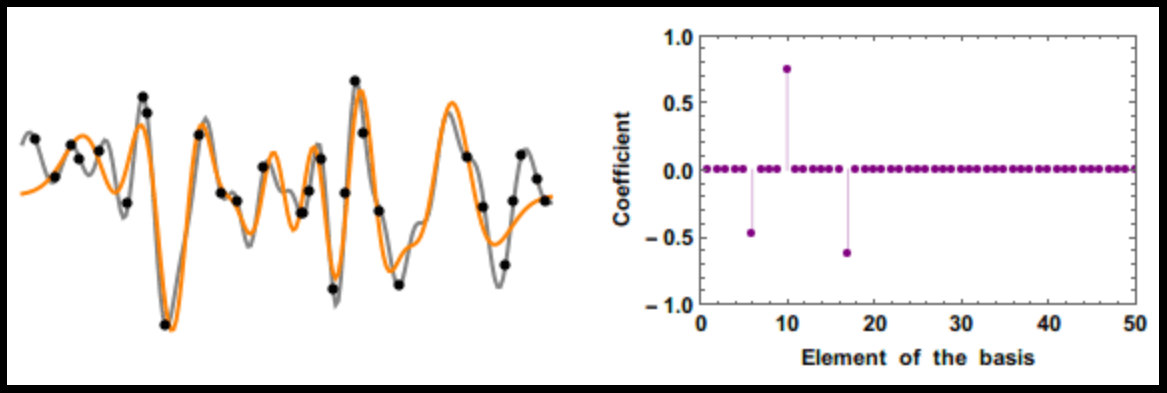
\includegraphics [width = \textwidth] {compressive-sensing.png}
\caption {
A conceptual illustration of compressive sensing.
(Retrieved from \href {commons.wikimedia.org/wiki/File:Orthogonal_Matching_Pursuit.gif} {Wikimedia Commons})
}
\end {figure}

Figure 1 shows a generic situation in which a signal is crowded in the given basis, but sparse in the transformed basis.
The black line on the left is the original signal, and the yellow line is the reconstruct signal.
If the signal is sparse on a certain new basis, as shown in the right, then for a good approximation, we may take only the largest components for reconstruction.

Generally speaking, compressive sensing aims to reconstruct an underdetermined linear system, when the sparsity of solution guarantees successful recovery for most cases.
More measurements are required to recover the signal in the nonsparse basis, while fewer suffice in the sparse basis.
But, even if we are sure that the sparse basis exists, its construction is another undertaking.
In our settings for hybrid beamforming structure, a way of generating the sensing matrix and pilot vectors in the estimation stage has to be devised and justified.

Compressive sensing approaches can be divided into two categories, the convex programming approach and the greedy approach \cite {RDD18}.
We will discuss one from each in more detail: Dantzig Selector and Orthogonal Matching Pursuit.

Let us say the number of model parameters \m {N_p \in \mathbb {N}} is much larger than the number of measurements \m {N_m \in \mathbb {N}}, that is,
%
\DispNum {N:p:Nm:Nm} {
N_p \gg N_m 
}
%
To start, consider \m {\V {x}, \V {x}' \in \mathbb {K} ^{N_p}} and \m {\M {Q} \in \mathbb {K} ^{N_m \D  N_p}}, and the linear system
%
\DispNum {y:y:Qx:Qx} {
\V {y}
=\M {Q} \V {x} 
}
Certainly, if \m {\M {Q} \RB {\V {x}_1 - \V {x}_2} = 0}, then \m {\V {x}_1, \V {x}_2} are indistinguishable.
But if \m {\V {x}} is sparse, can we rule out some of the possibilities?

To be precise, we say \m {\V {x}} is \m {s}-sparse, if only at most \m {s} components of \m {x} is nonzero.
We use subscript in square brackets, like \m {\mathcal {A}}, to denote extraction of components.
That is, if there is some \m {\mathcal {A} \subseteq \CB {0, \dots, N_p-1}} such that
%
\DispNum {x:A:x::x:} {
\V {x} _{\SB {\mathcal {A}}}
=\V {x} 
}
%
with
%
\DispNum {A:A:s::s:} {
\Nm {\mathcal {A}} \leq s. 
}

It is shown that in the noiseless case, a \m {\ell_1}-minimization program recovers the \m {N_p}-dimensional signal, with \m {N_m} measurements, under overwhelming probability \cite {Can05}.

As an application, it often occurs that a camera takes a high definition photo and compresses the image later.
But it may be desirable that a camera equipped with fewer sensors shall take a lower resolution photo to save storage, and recover the image later.
Such advantage can be useful in medical imaging, since it is not only expensive, but also harmful, to take too many images, and the accuracy is critical to the diagnosis too \cite {CaT07}.


\section {The Dantzig Selector}

If the linear system is moreover subject to noise \m {z},
%
\DispNum {y:y:Qx:xz} {
\V {y}
=\M {Q} \V {x} + \V {z} 
}
is it still possible to recover \m {\V {x}}?

We introduce some conventions.
For \m {\mathcal {A} \subseteq \CB {0, \dots, N_p-1}}, denote
%
\Disp {
\V {x}  _{\SB {\mathcal {A}}}
=&\sum _{i \in \mathcal {A}} \V {v} \V {u} _{i} \\
%
\M {Q}  _{\SB {\mathcal {A}}}
=&\sum _{i \in \mathcal {A}} \M {Q} _{\SB {:,i}} 
}
%
That is, respectively, the components of \m {\V {x}}, and the columns of \m {\M {A}}, that have indices in \m {\mathcal {A}}.

\Result
{Definition}
{
For fixed \m {s =0, \dots N_p -1}, we say that \m {\M {Q}} satisfies \m {\d_s}-restricted isometry property (hereafter \m {\d_s} RIP) of sparsity \m {s} with respect to \m {0 \leq \d_s \leq 1}, if for all \m {s}-sparse \m {\V {x}}
%
\DispNum {1:2:Qx:22} {
\RB {1-\d_s} \VNm {\V {x}} _2 ^2
\leq &\VNm {\M {Q} \V {x}} _2 ^2 \notag \\
%
\leq &\RB {1+\d_s} \VNm {\V {x}} _2 ^2 
}
}
%
It helps to think that \m {\M {Q}} is almost unitary up to relative error \m {\d_s}.

For concreteness, say \m {\V {z}} is an i.i.d.\ random normal vector.
If so, a stronger result was established that, with another \m {\ell_1} minimization program called Dantzig selector (hereafter DS), recovery under the noisy case is again possible.

\Result
{Algorithm}
{
\begin {itemize}
\item Input \m {\M {Q} \in \mathbb {R} ^{N_m \D N_p}} and \m {\V {y} \in \mathbb {R} ^{N_m}}.
%
\item Compute the convex program
%
\DispNum {h:h:mi:yg'} {
\hat {\V {h}}
\leftarrow \begin {cases}
\Min {\V {h}'} & \VNm {\V {h}'} _1 \\
%
\mathrm {subject} \; \mathrm {to} \quad & \VNm {\M {Q}^\dagger \RB {\M {Q} \V {h}' -\V {y}}} _\infty \leq \g \\
\end {cases} 
}
\item Output \m {\hat {\V {h}}}.
\end {itemize}
}

Algorithm [2] recovers \m {\V {x}} with the expected error norm bounded with overwhelming probability and is nearly optimal \cite {CaT07}.
The \m {\ell_1}-minimization problem with \m {\ell_\infty}-constraint may be recast as a linear program, for which techniques from convex optimization may be used, and Candès and Romberg provided an implementation on their website \cite {CaR05}.

Here the constant \m {\d_s} is significant, since we can't just take \m {\M {Q}} to be any unitary matrix, for which \m {\d_s =0}.
A common approach is choosing i.i.d.\ entries of \m {\M {Q}}, and it was established \cite {BDD08} that if \m {\VNm {\M {Q} \V {x}} _2} concentrates sharply, \m {\M {Q}} has RIP for overwhelming probability, but it remains to conceive an algorithm that efficiently generates RIP matrices.

Back to our problem of MIMO channel estimation, recall that, luckily, physical evidences suggest that mm-wave channels are sparse in the number of paths.
Bajwa et.\ al.\ \cite {BHS10} used DS, where they argued that if the \m {\ell_0}-norm of the channel matrix may be bounded by a constant, DS may be applied to estimate the time-dependent single-antenna channel response,
and in the accompanying note \cite {BHR08} they justified that \m {X} has RIP for overwhelming probability.
However, there seems to be no work by now which addresses the constraint of hybrid beamforming.

Some scholars applied least absolute shrinkage and selection operator (Lasso) instead.
In fact, it can be shown that Lasso and DS have similar behavior \cite {AsR10}.
Lian, Liu and Lau applied Lasso on MIMO with an analog combiner \cite {LLL17}.
Destino, Juntti, and Nagaraj used an adaptive Lasso \cite {DJN15}, and Vlachos, Alexandropoulos, and Thompson \cite {VAT19} used Lasso on hybrid beamforming with an additional random spatial sampling device.
Both Destino et al and Vlachos et al optimize formulate an algorithm to jointly find the channel and the sensing matrix, which can result in high complexity.

\section {Orthogonal Matching Pursuit}

At the same time, Tropp and Gilbert \cite {TrG07b} suggested likewise that a greedy algorithm called orthogonal matching pursuit (OMP) which also aims to reconstruct a sparse signal in an underdetermined system.
Again consider the situation of \eqref {y:y:Qx:xz}.

\Result
{Algorithm}
{
\begin {itemize}
%
\item Input \m {\M {Q} \in \mathbb {R} ^{N_m \D N_p}} and \m {\V {y} \in \mathbb {R} ^{N_m}}, \m {\eta >0}.
%
\item Initialize
%
\Disp {
\V {r}
\leftarrow &\V {y} \\
%
S
\leftarrow &\varnothing 
}
%
\item Start the loop with counter \m {i \leftarrow 1}.
%
\item Find
%
\DispNum {n:n:n0:nr} {
n
\leftarrow \underset {n' =0, \dots, N_p-1} {\mathrm {argmax}}
\Nm {\M {Q} _{\SB {:,n'}} ^\dagger \V {r}} 
}
%
and append \m {S \leftarrow S \cup {n}}.
%
\item Compute
%
\DispNum {Q:Q:QS:Qy} {
\M {Q} ^\ddagger
\leftarrow &\RB {\M {Q} _{\SB {S}} ^\dagger \M {Q} _{\SB {S}}} ^{-1} \M {Q} _{\SB {S}} ^\dagger \\
%
\V {r}
\leftarrow &\V {y} -\M {Q} _{\SB {S}} ^\dagger \M {Q} ^\ddagger \V {y} 
}
%
\item Break if
%
\DispNum {r:2:h':h'} {
\VNm {\V {r}} _2
<\eta 
}
%
otherwise, go to step 4.
%
\item Output 
%
\DispNum {g:g:Qy:Qy} {
\hat {\V {g}}
\leftarrow \M {Q} ^\ddagger \V {y} 
}
\end {itemize}
}
%
The columns of \m {\M {Q}} are chosen greedily, and we expect its columns to span \m {\V {x}}, playing a role similar to the sensing matrix of DS.
In each step, we estimate the noise \m {\V {r}}, and find a new column most correlated with it, to refine the estimation for \m {\V {x}}.
It is shown that the probability that OMP recovers \m {\V {x}} completely is overwhelming \cite {TrG07a}.

OMP has since been commonly used for channel estimation.
Alkhateeb, Leus, and Heath Jr.\ \cite {ALH15} examined the trade-off between number of measurement and accuracy for an all-phase-shifter beamforming matrix based on nonuniform fixed set of angles.
Hu, Wang, and He \cite {HWH13} applied OMP to estimate path delay of OFDM subcarriers.
Lee, Gil, and Lee \cite {LGL16} considered a hybrid system, where the hybrid beamforming matrix serves as sensing matrix;
the analog stage is a Fourier matrix, and the digital stage consists of a collection of columns vectors of a unitary matrix.
Gao, Dai, and Wang proposed a variant of OMP which there is the assumption of spatially common sparsity \cite {GDW15}.

Performance guarantee of OMP is also studied on various conditions.
Cai, Wang, and Xu \cite {CWX10} gave a new bound on performance of OMP under assumption of low coherence of columns.
Cai and Wang \cite {CaW11} extended the study to DS and other convex programs for sparse recovery, and Ben-Haim et.\ al.\ \cite {BEE10} followed up and refined their bounds, concluding that OMP is better for low SNR scenario, and DS is better for high SNR.

\section {Contribution}

Due to the constraint of hybrid structure, the designs which use fully digital beamforming cannot be directly applied, and the designs which use only analog beamforming might not be optimal.
Indeed, if DS is shown to be optimal \cite {CaT07}, then if we can overcome the problem of complexity among other difficulties, it may turn out to outperform greedy methods, and is even necessary for less ideal situations.

In this treatise, we consider a hybrid structure with a uniform linear array with both precoders and combiners on each side.
In chapter 2, we plan to generate random beamforming matrices, and use DS to estimate the channel in the space frequency domain.
To the best of our knowledge, the sensing matrix with i.i.d.\ entries in both analog and digital stages has not been discussed on the literature.
In chapter 3, we shall see that in our proposal, the effective sensing matrix has RIP for high probability, which may serve as the sensing matrix for DS,
and we give a quantitative bound (which holds for high probability) on the expected error norm.
In chapter 4, numerical results show that DS is superior to other methods for our problem.
Since DS is more accurate, it can be used when the sample is less sufficient and the noise level is higher, where it might be the case that only DS can recover successfully.
Considering its higher complexity, we remark that it can be cast as a linear program, and the basis pursuit denoising form may be used.

It appears that, for a given number of sampling, DS recovers better than OMP, except perhaps in high noise scenario.
Moreover, our setting is more general than Alkhateeb, Leus, and Heath Jr.\ \cite {ALH15} with only an analog combiner,
and our random generation of sensing matrix is simpler than Lee, Gil, and Lee \cite {LGL16},
and we do not rely on additional assumptions on sparsity as in Gao, Dai, and Wang \cite {GDW15}.

Our work is also an improvement to Bajwa et.\ al.\ \cite {BHS10}.
First, while their method takes many time slices, for our case a few time slices suffice, since the channel is time independent.
Second, with the further constraint of hybrid beamforming, the channel matrix is downsampled, it is unclear whether their guarantee for successful signal recovery is still valid.
Third, generating random sequences can lead to high complexity \cite {LGL16}, and we instead use random beamforming matrices.

In addition, it seems that with the same threshold, DS recovers better than Lasso, except perhaps in low noise scenario.
Again, our proposed method is more general than Lian, Liu and Lau \cite {LLL17} with only an analog combiner,
and our sensing matrix is generated more simply than in Destino, Juntti, and Nagaraj \cite {DJN15},
and we do not require special devices as in Vlachos, Alexandropoulos, and Thompson \cite {VAT19}.
Overall, it is clear that DS leads to a relatively better regularization than OMP and Lasso.

